%************************************************
\chapter{Active Motion}\label{ch:activeMotion}
%************************************************
\textit{Active motion} describes the process of converting energy resources into directed motion. Living beings performing active motion are \eg humans, animals, migrating cells, and microorganisms such as bacteria.

\graffito{The motion of a human floating in a sea is only subject to the current, however, by using energy and muscle power the human can swim and therefore move directed.}
While it is everyday experience that animals and humans are able to move directed, it is a nontrivial fact for microorganisms. Especially considering cells and bacteria which are often surrounded by fluids and therefore experience thermal \textit{diffusion}. The diffusion alone would lead to the so called \textit{Brownian motion}, a purely random motion named after its famous discoverer \citeauthor{brown:1828} and his studies on the motion of pollen particles \cite{brown:1828}. However, non-diffusive motion patterns have been observed for microorganisms in many experiments. \autoref{fig:migrationPaths} shows two examples of cells and bacteria for which directed and persistent motion has been recorded.

\begin{figure}[bth]
    \myfloatalign
    \subfloat[][]{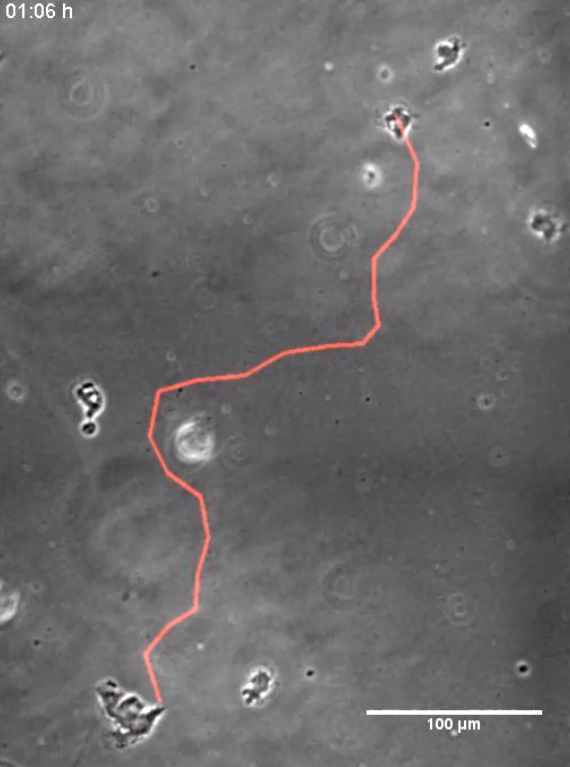
\includegraphics[width=.45\linewidth]{gfx/migrationCell}} \quad
    \subfloat[][]{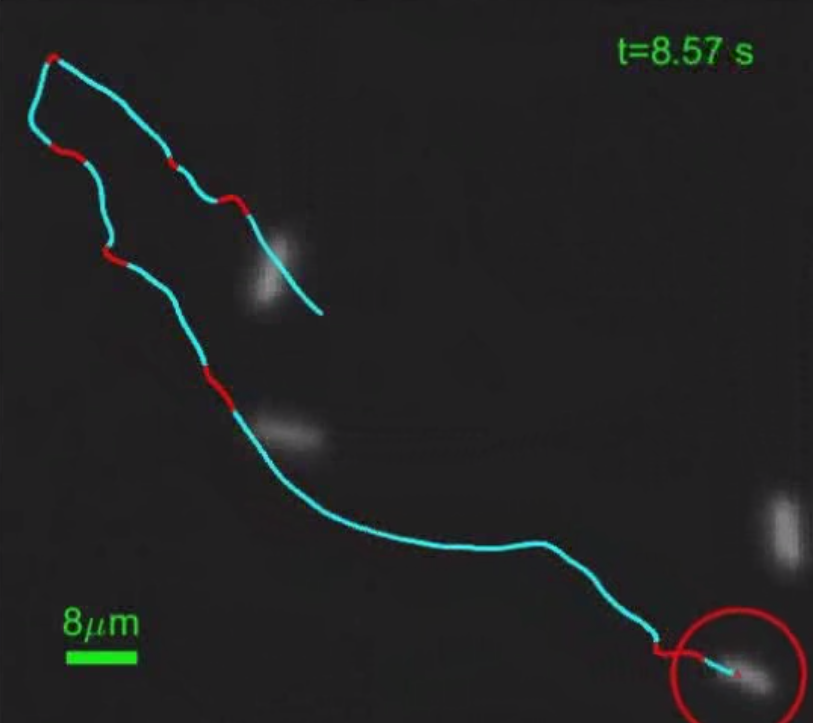
\includegraphics[width=.45\linewidth]{gfx/migrationBacillusSubtilis}}
    \caption[Directed, persistent migration paths]{Directed and piecewise persistent migration paths for (a) an immature bone marrow-derived mice dendritic cell \cite{maiuri:2015}, and (b) a Bacillus subtilis bacterium \cite{najafi:2018}.}\label{fig:migrationPaths}
\end{figure}

In the following, the main reasons and applications of active motion in biological environments are discussed, an overview of the related current research in different fields is presented, and the \textit{search problem} aspects are briefly introduced.

\section{Motivation and examples}\label{sec:MotAndExa}
The reasons for active motion are manifold and depend among others on the species and environmental conditions. \graffito{A mouse might need to hide or run from a fox while a human might be looking for lost keys.} They include, for example:

\begin{itemize}
 \item \emph{Survival}: evading predators, escaping hazardous locations, finding shelter.
 \item \emph{Foraging}: finding food or nutrients, hunting prey.
 \item \emph{Reproduction}: finding mates.
 \item \emph{Search}: searching for objects or locations of interest.
 \item \emph{Migration}: finding and exploring new habitats and environments.
 \item \emph{Biological tasks}: \eg morphogenesis, wound healing, immune response, etc.
\end{itemize}

From this list one can infer that most of the time a specific \emph{search problem} is the cause of active motion.
Furthermore, it is reasonable to assume that, depending on the motivation, also the movement patterns of active motion vary. To stick with the example of the mouse and the human: the movement pattern of a mouse running for its life certainly looks different from that of a human looking for its lost keys. Therefore, there is a lot of ongoing research with the goal of obtaining a qualitative and quantitative understanding of the many kinds of active motion. Considering the tasks and functions of cells and bacteria, understanding their migrational properties is especially relevant in the fields of biology and medicine.

To give an impression of the current research on search related problems, a few examples are presented below.

\subsection*{Humans}
For humans almost any activity in everyday life is connected to active motion (\eg doing groceries, sports, work, ...). However, on a macroscopic scale ancient migration and colonization can be also analyzed as active motion. In this sense, the colonization of America and the Neanderthal replacement in Europe has been studied \cite{flores:2007}. The total dispersal times as well as the effective velocity of dispersal, which have been derived within this study, are in good agreement with archeological data and the given reference values.

\subsection*{Animals}
\graffito{Here, the term animals includes all kinds of terrestrial animals, birds, fishes and insects.}
There is quite a lot of literature on active motion of animals such as the \mycitet{breed:2010} and the book \mycitet{breed:2012} which cover many interesting aspects such as \emph{search, navigation, migration, dispersal, foraging, self-defense, mating}, and many more in great generality. However, a wide range of research also focuses on very specific topics with most of them being focused on foraging behavior or other search problems requiring active motion or relocation.

\graffito{First animals were categorized into cruise and ambush searchers...}Based on the foraging behavior of animals, people first categorized them into \textit{cruise} and \textit{ambush} types \cite{greene:1983}. The animals of cruise type, such as tuna and soaring hawks, move around the environment and simultaneously search for food or prey. On the contrary, the animals of ambush type stay immobile for a long time until the prey approaches and enters their strike zone. Examples of animals of this type include herons and rattlesnakes.

Nonetheless, in a theoretical approach, \mycitea{andersson:1981} compared continuous travel to a search mode of alternating pause-and-travel in regard of energy consumption and prey detection efficiency. The results propose that, under given circumstances (prey density and detectability, energy expenditure during travel, etc.) a pause-travel tactic may become superior.

The studies of foraging in planktivorous fish \cite{obrien:1990} revealed that the searching behavior follows a pause-and-travel type of dynamics rather than a cruise or ambush strategy. This search pattern, called \textit{saltatory search} by \mycitea{evans:1988}, has been observed in many foraging species. Even the movement of the human eye during the process of reading, as the eye shifts focus along a line of type \cite{huey:1968} or finding a specific letter sequence \cite{chase:1986}, can be described in such a saltatory manner. It is even possible to assign a kind of saltatory search to the animals such as soaring hawks, which are traditionally categorized as cruise searchers. \graffito{... whereas later on they were classified using a continuum in-between both extremes.}The reason is that their eye movements can be locked in to scan an area for preys before switching to a new region. Therefore, the saltatory search serves as an explanatory tool and supposedly all search behavior can be placed on a saltatory continuum with the extremes being the cruise and the ambush search \cite{obrien:1990}.

Indeed, the saltatory motion has given rise to a lot of research up to today.\graffito{The mentioned movement pattern has had many names in biophysics literature, namely saltatory search, intermittent locomotion, intermittent search, stop-go running, stop-and-go swimming, pause-travel locomotion, ...} Observations of white crappie revealed alterations in speed, travel distance and pause times when feeding on prey of different sizes \cite{obrien:1989}. These adaptions were analyzed with regard to efficiency using a net energy gain simulation model and the results are believed to have considerable generality for other saltatory animals.

\mycitea{kramer:2001} propose the term \textit{intermittent locomotion} to describe the observed stop-and-go motion. They showed that despite the fact that pausing adds acceleration and deceleration phases to locomotion, which are costly in terms of energy usage, it is still widespread among diverse species and can have benefits such as recovery from fatigue, improved detection of prey, predators and travel routes, and reduced detection by other organisms.

Juvenile plaice (\textit{Pleuronectes platessa}) change their predatory behavior and motion upon the discovery of a potential prey during search \cite{hill:2000}. Performing several moves before an attack, while the distance of moves is decreased, gives rise to the assumption that plaices detect their prey more efficiently when stationary than while moving. Furthermore, the pauses between moves are shortened and the rate of turning per unit distance is increased.

Naturally, mathematical approaches and models describing saltatory or intermittent motion of animals have also emerged over the years, which will be briefly discussed in \autoref{ch:randomSearchStrategies} (also see \eg \cite{reynolds:2006, benichou:2011}).

Besides the saltatory search research, which is a topic to fill a whole book alone, there have been further relevant studies, \eg along the following lines:
\begin{itemize}
 \item A study on the depth vision and perception of the three-dimensional environment of a toad \cite{lock:1979} revealed that in presence of a prey, the toad plans its route before starting to move and that the route is preprogrammed, meaning that once the toad has started moving, it does not correct its path even if the prey has relocated.
 \item Life cycle specific movements are a widespread phenomenon among many marine species \cite{pittman:2003} such as fish and decapod crustaceans and happen at a broad range of spatial and temporal scales. Because these scales are not considered in many traditional studies of animal-environment relationships they underlie scale-related limitations. The authors therefore argue that this needs to be considered in the process of designing sampling strategies. Furthermore, they offer a conceptual framework which addresses scale and environmental heterogeneity. The awareness of these concepts may not only help in improving studies but also in counteracting the overexploitation of marine animals, which is a severe global threat to marine life and environment with no foreseeable solution in the near future.
 \item The control and function of counterturning (succession of alternating left and right turns), a feature in the flight of insects following a wind-borne odor, was discussed \cite{kennedy:1983} as there was unambiguous evidence only for the findings concerning a certain flying male moth. Furthermore, the main function of counterturning appeared to be the redetection of an already perceived elusive odor.
 \item Radiotagged red squirrels (\textit{Sciurus vulgaris}) have been observed in coniferous and deciduous habitats in regard to activity pattern, activity budget and foraging behavior \cite{wauters:1992}. Food availability, food choice and feeding rate are then used to explain differences between habitats.
 \item The prey-capture techniques and prey preferences of six different ant-eating jumping spiders (\textit{Saliticidae}) have been studied in the laboratory \cite{jackson:1992}. The results on the predatory behavior as well as the preference for ants are discussed in consideration of the findings on other ant-eating spiders.
\end{itemize}
The observed motility patterns in biological environments are not limited to macroscopic scales. As we will discuss below, similar dynamical behavior is frequently observed on microscopic scales as well.

\subsection*{Microorganisms}
Directed and persistent motion has also been observed for microorganisms as it was stated before and shown in \autoref{fig:migrationPaths}. Considering the diverse tasks and functions of different microorganisms, this is not surprising as diffusive Brownian motion is highly inefficient in most (search) applications.

Understanding cell migration is of utmost importance as it has essential functions (not only) in the human body in regard to diverse health concerns. This importance is emphasized in many of the mentioned references below. Therefore, in the past 30 years there has been a focus on understanding migrational processes of cells and bacteria, the underlying mechanics and their properties, of which some excerpts are presented here.
\begin{itemize}
 \item %1992
 The migration of different \textit{E. coli} strains on glass and solid surfaces differing in charge and hydrophobicity was studied in an \vitro system in order to gain insight on catheter-associated bacteriuria \cite{harkes:1992}. The findings propose that prevention strategies should be based on inhibition of bacterial growth rather than on modifying the physicochemical properties of the catheter surface.
 \item %1996- 2003 
 There are many articles around which focus on explaining the mechanics, molecular processes and dynamics involved in cellular motion \cite{mitchison:1996,lauffenburger:1996,horwitz:1999,horwitz:2003}. Some topics covered include contractile forces and adhesion, the role of actin filaments and the cytoskeleton, polarization of the cell, molecular stimulation, membrane extension, and many others.
 \item %1999 
 In a study on the directional sensing of \textit{Dictyostelium discoideum} amoebae it is concluded that the cell senses direction by spatial regulation of the activity of the signal transduction pathway \cite{parent:1999}.
 \item %2009 
 The specific mechanisms and factors that promote directionally persistent as opposed to random cell migration are identified and examined \cite{petrie:2009}.
 \item %2011
 In a study of cell motility a mathematical model is developed, which makes use of the analysis of live cell image sequences in order to gain information about collective biomechanical and molecular mechanisms of cell motion, such as \eg molecular structures, dynamics, processes within the cell, and many more \cite{coskun:2011}. Therefore, this model is supposed to allow drawing conclusions from the analysis of the cell motion alone.
 \item %2015
 In regard to the medical issue of removing infected prostheses from patients, bacterial cell migration has been observed and studied \cite{spector:2015}. For the migration from a colonized to a sterile plate, yeast and \textit{Staphylococcus aureus}, which belongs to the bacteria that are responsible for most hospital infections, have been used. They believe that infected prostheses in patients can be completely cleaned by this method in the near future.
 \item %2015
 The coherence of cell migration speed and cell persistence is shown based on experimental data \vitro and \vivo \cite{maiuri:2015}. Additionally, using a theoretical model a generic phase diagram of cell trajectories is obtained which represents the whole range of observed migration patterns.
 \item %2015
 In a preview, the distinct motility modes exhibited by migrating cells and their ability to switch between modes according to physical or chemical cues is discussed \cite{welch:2015}.
 \item %2016
 It is physiologically reasonable that cells move through crowded and complex environments, typically in three-dimensional fibrillar networks \cite{mak:2016}. A review on the progress of understanding single-cell migration through such environments is given.
\end{itemize}
 We will take a brief look at search-related studies in nonliving systems in the following.
 
 \subsection*{Artificial particles}
 Inspired by microorganisms researchers have developed artificial self-propelled active particles with similar properties and behavior in regard to motility. These could turn out to be very useful in many fields such as \eg health care, sustainability, and security.
 
 In a review, the development of artificial self-propelled micro- and nanoparticles, their application to the study of nonequilibrium phenomena, and open challenges are discussed \cite{bechinger:2016}. While doing so the focus lies on the basic physical features of the interactions with crowded and complex environments.
 
\bigskip
 
\noindent At this point it is worth emphasizing again that many of the given examples for active motion deal with search problems and in the course of evolution, as an answer, the creativeness of Mother Nature has yielded many different search types and strategies which will be partly addressed later on. Hence, understanding their main qualitative and quantitative properties is beneficial to many fields of research and will be a main focus of this work.



%*****************************************
%*****************************************
%*****************************************
%*****************************************
%*****************************************
